\documentclass{article}

\usepackage{amsmath, amsthm, amssymb, amsfonts}
\usepackage{thmtools}
\usepackage{graphicx}
\usepackage{setspace}
\usepackage{geometry}
\usepackage{float}
\usepackage[utf8]{inputenc}
\usepackage[english]{babel}
\usepackage{framed}
\usepackage[dvipsnames]{xcolor}
\usepackage{tcolorbox}
\usepackage{listings}
\usepackage{hyperref}

\colorlet{LightGray}{White!90!Periwinkle}
\colorlet{LightOrange}{Orange!15}
\colorlet{LightGreen}{Green!15}

\newcommand{\HRule}[1]{\rule{\linewidth}{#1}}

\declaretheoremstyle[name=Theorem,]{thmsty}
\declaretheorem[style=thmsty,numberwithin=section]{theorem}
\tcolorboxenvironment{theorem}{colback=LightGray}

\declaretheoremstyle[name=Proposition,]{prosty}
\declaretheorem[style=prosty,numberlike=theorem]{proposition}
\tcolorboxenvironment{proposition}{colback=LightOrange}

\declaretheoremstyle[name=Principle,]{prcpsty}
\declaretheorem[style=prcpsty,numberlike=theorem]{principle}
\tcolorboxenvironment{principle}{colback=LightGreen}

\setstretch{1.2}
\geometry{
    textheight=9in,
    textwidth=5.5in,
    top=1in,
    headheight=12pt,
    headsep=25pt,
    footskip=30pt
}

\lstset{
    language=Haskell,      % Linguagem do código
    basicstyle=\ttfamily,  % Fonte monoespaçada
    keywordstyle=\color{blue}, % Cor para palavras-chave
    commentstyle=\color{gray}, % Cor para comentários
    stringstyle=\color{green}, % Cor para strings
    breaklines=true,       % Quebra de linha automática
    frame=single,          % Coloca uma caixa ao redor do código
}

% ------------------------------------------------------------------------------

\begin{document}

% ------------------------------------------------------------------------------
% Cover Page and ToC
% ------------------------------------------------------------------------------

\title{ \normalsize \textsc{}
		\\ [2.0cm]
		\HRule{1.5pt} \\
		\LARGE \textbf{\uppercase{Relatório do trabalho 3 \\ Análise sintática e geração de código para ferramenta de documentação para linguagem Imp}
		\HRule{2.0pt} \\ [0.6cm] \LARGE{BCC328 - Construção de compiladores I} \vspace*{6\baselineskip}}
		}
\date{}
\author{\textbf{Autores:} \\
		22.1.4104 - Matheus Peixoto Ribeiro Vieira\\
		22.1.4022 - Pedro Henrique Rabelo Leão de Oliveira\\
		Semestre 24.2}

\maketitle
\newpage

% ------------------------------------------------------------------------------

\section{Introdução}
    Para o terceiro trabalho prático da disciplina Construção de Compiladores I, é solicitada a implementação do analisador semântico para a linguagem Lang, assim como a geração de código para Python e para a SVM.

\section{Modificações do trabalho 2 para o 3}
    Inicialmente, para o desenvolvimento do trabalho 3, focamos na incrementação do interpretador, permitindo o uso de arranjo e composição. Assim, foi possível a implementação correta dos métodos de ordenação solicitados e de algumas estruturas de dados. 

    
\section{Analisador semântico}
    Para o analisador semântico, foi utilizado um tipo algébrico com campos representando o contexto em que o programa é executado. Esse contexto contém 3 campos: um que armazena variáveis declaradas e seus respectivos tipos, outro que armazena as funções definidas no programa, guardando seu nome, uma lista de parâmetros com seus tipos e os tipos de retorno definidos, e um último que armazena os registros e seus campos internos. Optamos por não armazenar operadores no contexto e fazer a verificação dos mesmo através de funções que lidam com expressões e com suas possíveis regras. Para representar os erros, foi definido um tipo Error possuindo construtores para representar diferentes possibilidades de erro, como tipos incompatíveis, variável indefinida, função indefinida, registro indefinido, argumento de uma função sem valor atribuído em uma chamada, valor passado em uma chamada de função em que a mesma não possui nenhum argumento em sua definição, declaração repetida e números de retornos diferentes do que foi definido na declaração de uma função.

    Para iniciar a análise semântica, o analisador recebe a árvore sintática abstrata (AST) do programa vinda do analisador sintático, iniciando pelo tipo Prog que se dá por uma lista de definições, estas que podem ser novos registros ou funções. Com isso, cada definição é analisada e o contexto modificado a partir delas. Ao final, é verificado se existe a função main no contexto, uma vez que todo programa precisa ter a main implementada.

    \begin{lstlisting}
tcDefs :: Ctx -> [Def] -> Check ()
tcDefs ctx [] =
  let functions = [(func, (params, returns)) | (func, params, returns) <- funcs ctx]
  in
  case lookup "main" functions of
    Just _ -> Right ()
    Nothing -> undefinedFunction "main"
tcDefs ctx (d : ds) =
  case tcDef ctx d of
    Left err -> Left err
    Right ctx' -> tcDefs ctx' ds
    \end{lstlisting}

    Na definição de um novo registro ou de uma nova função, é sempre verificado se já não existe nenhum outro com mesmo nome, e da mesma forma é feito com os campos do registro. No caso de um novo registro, após essa verificação, o mesmo é inserido no contexto no campo de registros do programa com seus respectivos campos. Já quando se trata de uma função, criamos um contexto semelhante ao atual, entretanto inserimos a declaração dessa função no campo de funções do contexto e inserimos seus argumentos com seus tipos no campo de variáveis. Com isso os comandos dentro da mesma são analisados um por um a partir desse novo contexto. Por fim, caso a análise dos comandos retorne Right, ou seja, não retorne nenhum erro, o contexto com a nova função inserida nele, mas com o campo de variáveis vazio, é passado para a análise da próxima definição. Dessa forma, o escopo das variáveis é preservado, sem que as variáveis instanciadas em uma função seja conhecida em outra função. Do mesmo jeito, quando se trata do if-else ou do iretate, comandos em que dentro dele existe um bloco de código com escopo próprio, analisa-se comando por comando através do contexto do programa, mas quando passa para a análise do comando seguinte considera-se o contexto no estado em que ele estava antes do bloco de código, ignorando o novo contexto retornado, uma vez que na análise de comandos chamamos recursivamente uma função para analisar a lista de comandos e essa função vai passando o contexto sempre para a análise do comando seguinte.

    \begin{lstlisting}
tcCmd ctx (CmdIterate e c) =
  case tcExp ctx e of
    Right (BType TInt) ->
      case tcCmd ctx c of
        Left err -> Left err
        Right _ -> Right ctx
    Right ty -> incompatibleTypes (BType TInt) ty
    Left err -> Left err
    \end{lstlisting}

    Na análise de expressões, um caso particular é quando temos a expressão ENull que representa o valor nulo. Para ela, optamos por retornar o Right acompanhado do tipo (BType (TID "null")), para que assim, quando analisamos os comandos de atribuição ou de declaração em que ocorre uma atribuição no mesmo, podemos comparar se a atribuição é feita com o mesmo tipo da variável em questão ou com o valor nulo. Essa foi uma forma que definimos para representar o valor nulo, já que esse valor não tem um tipo específico como por exemplo um número ou um caracter, além de que "null" é uma palavra reservada na linguagem, e, portanto, não poderia ser usado com outro objetivo a não ser esse, logo podemos fazer isso sem nenhuma possibilidade de erro.

    Por último, outro caso particular de nosso projeto se dá na análise das regras dos operadores binários ou de comparação. Para isso, implementamos uma função para cada um dos dois casos, em que nelas, através de uma outra função auxiliar retirada do código de exemplo da linguagem Imp, testamos todas as combinações possíveis para os tipos esperados nas expressões do lado esquerdo e no lado direito do operador. Caso nenhuma combinação possível seja encontrada, é retornado um Left com os erros acumulados mostrando todas as possibilidades de tipos esperadas e as encontradas.

    \begin{lstlisting}
tcBinOpNumerico :: Ctx -> Exp -> Exp -> Check Type
tcBinOpNumerico ctx e1 e2 = 
  case tcBinOp ctx (e1, BType TInt) (e2, BType TInt) (BType TInt) of
    Right ty -> Right ty
    Left err1 ->
      case tcBinOp ctx (e1, BType TFloat) (e2, BType TFloat) (BType TFloat) of
        Right ty -> Right ty
        Left err2 -> 
          case tcBinOp ctx (e1, BType TInt) (e2, BType TFloat) (BType TFloat) of
            Right ty -> Right ty
            Left err3 -> 
              case tcBinOp ctx (e1, BType TFloat) (e2, BType TInt) (BType TFloat) of
                Right ty -> Right ty
                Left err4-> Left (err1 ++ err2 ++ err3 ++ err4)
    \end{lstlisting}
   
\section{Geração de código Python}

    Python é uma linguagem conhecida por não ser tipada, diferente de Lang. Em grande parte da geração de código, isso não é um problema, todavia deve ser verificado durante a leitura de dados, uma vez que Python lê qualquer entrada e a armazena como String. Dessa forma, uma variável x que, inicialmente deveria receber o valor \verb|10|, receberá \verb|"10"|, gerando erros em operações matemáticas.

    Para evitar que esse tipo de problema ocorresse, de forma similar ao que foi feito para o interpretador, aqui também é criado um ambiente chamado Env, que armazena uma lista de tuplas com ID e Type, indicando o nome da variável e o seu tipo. Assim, sempre que é identificado um comando de declaração (CmdDecl), esse ambiente é atualizado inserindo a nova variável.

    Então, quando uma leitura é realizada, é verificado o tipo da variável que irá recebê-la para que seja feito o \textit{casting} adequado, circundando o \verb|input()| com tal valor. Como o python não possui um casting direto para Python, foi utilizado um \verb|eval()|, e o mesmo ocorre para quando é algum item de uma composição. Dessa forma, nestes casos, quando se trata de uma string, é necessário passar, na linha de comando, durante a leitura, as aspas. Outros valores serão devidamente avaliados pelo Python.

    Em Lang, o retorno de uma função pode conter zero ou mais valores, assim como em Python. No entanto, em Lang, qualquer retorno dentro de uma expressão é tratado como um arranjo, mesmo quando apenas um único valor é retornado. Como consequência, sempre que uma função retorna um único valor, uma vírgula é adicionada ao final da linha, garantindo que o retorno seja interpretado como uma lista de valores em Python. Isso permite que os elementos sejam acessados por índices, assim como em Lang, facilitando a tradução do código entre as linguagens. Logo, toda chamada de função com um único valor de retorno deve ser tratada como uma expressão no código Lang, a fim de garantir consistência na tradução.

    Em Lang, dados complexos são conhecidos como composição, já em Python, eles são traduzidos para classes. Todavia, ao iniciar o item em Lang, são atribuídos valores padrões de acordo com o tipo, que seria o valor None em Python. Então, na tentativa de manter o padrão, os construtores das classes atribuem os valores padrões, como pode ser observado na figura \ref{fig:mapeamentoRacional}. 

    \begin{figure}[!htb]
        \centering
        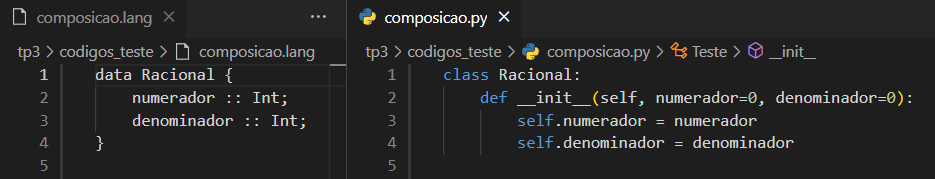
\includegraphics[width=1.0\linewidth]{dataRacionalMapeado.png}
        \caption{Mapeamento do data Racional para a classe Racional}
        \label{fig:mapeamentoRacional}
    \end{figure}

    Entretanto, devido à forma de como o Python funciona, problemas aparecem quando uma classe possui o valor de outra ou faz referencia a ela mesma de forma recursiva, como ocorre na figura \ref{fig:mapeamentoTeste}. Em Python, não é possível que t1 da classe Teste receba como valor padrão uma instância de Teste, dessa forma, o valor padrão deverá ser None. Logo, foi adotado o padrão de que o valor padrão para todas as composições fossem None, garantindo uma maior consistência na geração do código.

    \begin{figure}[!htb]
        \centering
        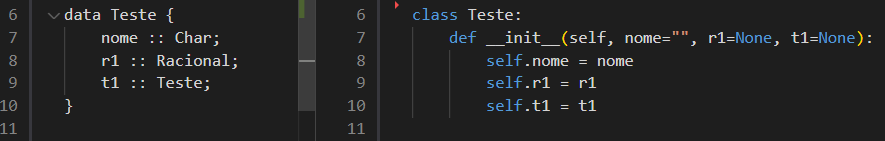
\includegraphics[width=1\linewidth]{mapeamentoDoTeste.png}
        \caption{Mapeamento do data Teste para a classe Teste}
        \label{fig:mapeamentoTeste}
    \end{figure}

\section{Geração de código SVM}

    Devido às dificuldades na implementação de outros componentes da Lang, somadas a erros que exigiram um tempo maior para correção, a geração de código para SVM não pôde ser realizada.

\section{Limitações do Nosso Compilador de Lang}

    Um problema que não foi solucionado em relação ao interpretador da Lang está no uso de arranjos dentro de composições. Todavia, eles são corretamente analisados pelos analisadores sintáticos e pelo analisador semântico, possibilitando a geração do código Python equivalente e funcional, sendo evidenciado pela implementação das estruturas de dados solicitadas, como pode ser observado na fila e na pilha.

    Ademais, outra limitação está na tradução do código Lang para Python, mais especificamente na divisão de números. Na Lang, a divisão entre dois inteiros, sempre resulta em outro inteiro, independente dos valores, o que não ocorre em Python, que pode resultar em um Float. 

    Assim, seria necessário circundar uma divisão com a função \verb|int()| ou realizá-la com o \verb|//|. Todavia, diferentes formas de implementar essa funcionalidade foram testadas, mas não foi possível obter uma solução final que geraria este comportamento, ocasionando tal limitação da tradução.

\section{Compilação e execução}
    Para auxiliar no desenvolvimento do trabalho, foi utilizado o cabal. Dessa forma, para compilar o código, é necessário escrever somente "cabal build lang".

    Para a execução do código, expandindo a execução por linha de comando, usamos como base o código abaixo e, onde encontra-se <opcao>, podemos escolher entre "lexer" (para executar somente o analisador léxico), "recursive-tree" (para exibir a árvore abstrata de sintaxe), "lalr" (executa o analisador léxico, o parser LALR e o interpretador), "peg" (executando o peg ao invés do lalr), "typed-interp" (executa a análise semântica entre o LALR e o interpretador), "typed-python" (executa a análise léxica, sintática com o LALR, semântica e, por fim, converte o código para Python) ou "typed-vm" (não implementado, gerando uma mensagem de erro). 

    \begin{tcolorbox}[title=Execução do interpretador, width=\linewidth, fontupper=\ttfamily,  halign=flush left, label = box:recursive]
      cabal run lang -- --<opcao> codigo.lang
    \end{tcolorbox}

    
\section{Conclusão}
    Com a conclusão do desenvolvimento deste trabalho, os conceitos para a construção de um compilador como um todo, como por exemplo o analisador léxico, sintático e semântico, foram explorados e solidificados, ao mesmo tempo em que aprimoramos nossa lógica de programação em Haskell. Embora não tenha sido possível entregar o código em sua totalidade, alcançamos avanços significativos.

    Ao refletirmos sobre o desenvolvimento da Lang como um todo, percebemos uma maior familiarização com a linguagem e com o paradigma funcional, além de um notável aprimoramento em nossa capacidade de resolução de problemas. Esse projeto foi, possivelmente, um dos mais complexos e desafiadores que enfrentamos até o momento em nossa graduação.

\newpage


\end{document}
